

\chapter*{1 Introduction}
\label{intro}
\addcontentsline{toc}{chapter}{1 Introduction}
\setcounter{chapter}{1}
\setcounter{section}{0}

Before digesting the content of this project, it is important to note that all abbreviations can be found in \textbf{\nameref{listAbr}}. All abbreviations are click-able links that will navigate to the relevant part of the document. File extensions are similarly linked and found in \textbf{\nameref{listExt}}. All internal links to relevant chapters are indicated in bold.
\section{Problem statement}
\label{ps}
%In order to solve the problem as stated in the \color{blue}introduction\color{black}, a solution that allows \hyperref[listAbr]{ARM}-type processors to be mimicked on standard \hyperref[listAbr]{PC} processors is needed. Since most \hyperref[listAbr]{PC}s make use of either intel\textsuperscript{{\tiny{\textregistered}}} or AMD\textsuperscript{{\tiny{\textregistered}}} \hyperref[listAbr]{CPU}'s (which are x86 based architectures - an ubiquitous iteration of \hyperref[listAbr]{CISC}), emulation or simulation is indeed required. This is because, on a machine level, \hyperref[listAbr]{CISC} architecture is incompatible with \hyperref[listAbr]{RISC} assembly language.
%It has been established that \hyperref[listAbr]{RISC} architecture will be mimicked on \hyperref[listAbr]{CISC} machines in order to evaluate student code. The degree of mimicry needed depends largely on the application. Whilst emulation mimics a pertaining architecture relatively closely, simulation does so more loosely. Emulation attempts to duplicate one device as accurately as possible in another environment. Simulation, by contrast, is not concerned with low-level duplication of devices, but instead mimics high-level behaviour.\cite{Chris}
%In the following chapters, both emulators and simulators will be evaluated as plausible solutions to the problem: \textbf{How can various student generated C and ARM language assembly code, compiled for RISC architectures, be tested on a single x86 (CISC) architecture PCs?}

As can be inferred from the title of this document, a process whereby computer system practical assessments can be assessed, in a relatively autonomous way, is required. It can be seen, when referring to the pertaining Stellenbosch Faculty of Engineering documentation, that a key aspect of the module group known as computer systems, has to do with embedded design. \cite{Stelle2020}
\\\\
This poses several challenges when it comes to the autonomous assessment of these modules. The code created by students to program microprocessors and embedded systems in general vary greatly. This makes the existence of a system, whereby all code can be assessed quickly and autonomously, quite difficult. A novel solution is thus required and of great interest.
\\\\
It is known that most embedded systems make use of a \hyperref[listAbr]{MCU}. Furthermore, in industry, ARM based \hyperref[listAbr]{MCU}s are ubiquitous and will, therefore, be the focus of this project. This poses another unique challenge in that the assessment of the aforementioned practicals are done by lecturers on standard \hyperref[listAbr]{PC}s. Since most \hyperref[listAbr]{PC}s make use of either intel\textsuperscript{{\tiny{\textregistered}}} or AMD\textsuperscript{{\tiny{\textregistered}}} \hyperref[listAbr]{CPU}'s (which are x86 based architectures - an ubiquitous iteration of \hyperref[listAbr]{CISC}), emulation or simulation is indeed required. This is because \hyperref[listAbr]{ARM} based MCU make use of \hyperref[listAbr]{RISC} instruction sets. On a machine level, \hyperref[listAbr]{CISC} architecture is incompatible with \hyperref[listAbr]{RISC} assembly language.
\\\\
It has been established that \hyperref[listAbr]{RISC} architecture will be mimicked on \hyperref[listAbr]{CISC} machines in order to evaluate student code. The degree of mimicry needed depends largely on the application. Whilst emulation mimics a pertaining architecture relatively closely, simulation does so more loosely. Emulation attempts to duplicate one device as accurately as possible in another environment. Simulation, by contrast, is not concerned with low-level duplication of devices, but instead mimics high-level behaviour.\cite{Chris}
\\\\
A two-part problem therefore exists when it come to the assessment of computer system (and related modules) practicals in an autonomous way:
\\\\
\textbf{How can greatly varying student generated C code, compiled for RISC architectures, be tested on a single x86 (CISC) architecture PC while maintaining student created MCU configurations?}
\\\\
Figure ~\ref{fig:introDia} illustrates the pertaining code as part of the embedded design process that is of interest to this project. This is the C code that will be analysed to facilitate automation of the task alluded to in the problem statement. Lastly, modules called Digital Design and Electronic Design are also provided by the Stellenbosch Faculty of Engineering \cite{Stelle2020}. These modules are also taken into account when creating the system which is the focus of this project.
\begin{figure}[H]
\begin{center}
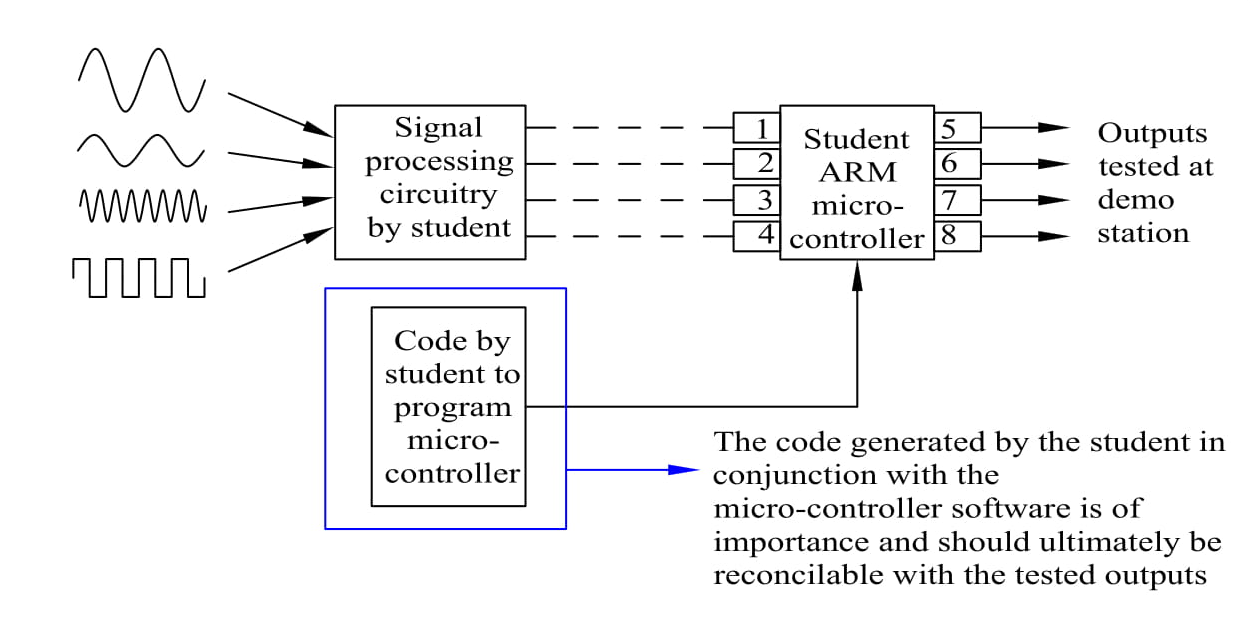
\includegraphics[width = 100mm]{diagram1.png}
\caption{Pertaining part of the embedded design process}
\label{fig:introDia}
\end{center}
\end{figure}

\section{Objectives}
\label{obj}
The objectives of this project are aligned so as to address the problem statement as highlighted in \textbf{1.1 \nameref{ps}}. If these objectives are convincingly  met, the problem statement will subsequently have been addressed.
\\\\
Due to the two-part nature of the problem described, the main objectives are hence outlined.
\subsection{Emulator/simulator investigation}
\label{emInvestObj}
The tasks required by students, enrolled in the various Design and Computer Systems modules, are greatly varying and are done on a wide variety of ARM based MCUs. Due to the varying range of ARM processors (which the scope of this project has been narrowed to, due to their ubiquity) a robust solution is not readily apparent.
\\\\
It is thus an objective of this project to investigate existing emulators/simulators to assess the degree to which they are suitable for solving the problem as stated in \textbf{1.1 \nameref{ps}}.
\subsection{Autonomous high-level code structure evaluation}
\label{highLevObj}
As a second objective it is necessary, for automation, that student code be assessed. Once a suitable emulator/simulator has been identified, the emulator/simulator (depending on its degree of fidelity) needs to be compatible with many different code based approaches to tasks given by practical assessments.
\\\\
Indeed, due to the nature of coding, once a problem needs to be solved in Design and Computer Systems modules by students, greatly varying approaches will be taken. This is a side-effect of any creative endeavour. The second objective is thus to address this issue. Student code must be autonomously reconciled with a chosen emulator.

\section{Summary of work}
\label{sow}

\color{green} This will be done when the report is finished\color{black}

\section{Scope of project}
\label{scOfWrk}
Due to the complex, dynamic nature of the problem at hand (autonomous assessment of C code, compiled for RISC architecture, evaluated on CISC machines) as described in \textbf{1.1 \nameref{ps}}, the scope needs to be narrowed. 
\\\\
It can be seen in \textbf{\nameref{2emul}} that simulators are a more wide-spectrum solution. Architecture can be mimicked for a much wider range of MCUs. Emulators, however, are of greater specificity and since these are preferred over simulators (due to their higher degree of fidelity), the choice of emulator greatly narrows the scope. It will be seen in   \textbf{\nameref{2emul}} that the scope was narrowed to mimicking the STM32F4 family of \hyperref[listAbr]{MCU}s. The reasons for this, are also illustrated in \textbf{\nameref{2emul}}.
\\\\
As for the problem of automated high-level code evaluation, it can be more eloquently addressed by focusing on specific solutions rather than general ones. This was done by automating the evaluation using the Python programming language. It has been mentioned that \hyperref[listAbr]{PC}s will be used as the host platform of any ARM emulation/simulation. This constraint is inherent to the task and narrows the host operating system to either Windows, Linux and MacOS.
\\\\
Since most people use Windows, as shown by StatCounter Global Stats and illustrated in \textbf{\nameref{C}}, the scope is further narrowed to Windows \hyperref[listAbr]{PC}s. It is important to note that Python 3 is a cross-platform programming language and can run on other operating systems as well. Any of the programs written as part of this project, will thus work on any machine with Python 3 installed with a very important caveat: The required modules must be installed on the machine. The required modules can be seen in the code displayed in \textbf{\nameref{D}}.
\\\\
To increase the level of automation, the problem of having to install python and specific modules must be avoided. Since the scope has already been narrowed to focus on Windows \hyperref[listAbr]{PC}s a solution has been chosen that involves a simple Windows .exe files. This allows the programs written as part of this project to run on any Windows \hyperref[listAbr]{PC} regardless of whether Python 3 is installed or not.
\\\\
Moreover, we will see that the chosen emulator only supports certain STM32 boards. Although this does constrain the fidelity of the solution somewhat, it does not diminish the completeness of the solution. It will be seen in \textbf{\nameref{2emul}} that \hyperref[listAbr]{MCU}s belonging to the same family of STM32 devices can be emulated on each other somewhat, since they share a \hyperref[listAbr]{HAL} library.
\\\\
Lastly, it is beyond the scope of this project to emulate the full functionality of any \hyperref[listAbr]{MCU}. No emulator is of such high fidelity that it supports a full range of peripherals whilst maintaining real-time code execution. The objective, bearing the aforementioned in mind, thus becomes to show that some functionality can indeed be emulated. It is assumed that the illustration of this objective (emulating one specific function) will highlight that atleast some, if not all, functionality can be replicated in an emulated environment. The chosen functionality is to blink an LED on the emulated \hyperref[listAbr]{MCU} using code generated in STMCubeIDE for a real \hyperref[listAbr]{MCU} within the same family. 

\section{Roadmap}
\label{rdmap}

\color{green} This will be done when the report is finished\color{black}
